\documentclass[border=10pt]{standalone}
\usepackage{tikz}

\begin{document}
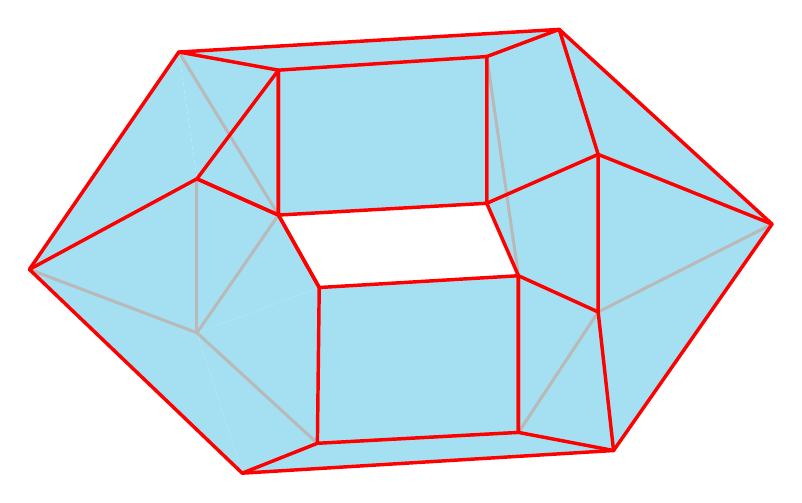
\begin{tikzpicture}[scale=1.15,line join=round,line cap=round]
    \definecolor{facecyan}{RGB}{164,224,242}

    \coordinate (L)  at (0.00,2.35);
    \coordinate (TL) at (1.65,4.75);
    \coordinate (TR) at (5.85,5.00);
    \coordinate (R)  at (8.20,2.85);
    \coordinate (BR) at (6.45,0.35);
    \coordinate (BL) at (2.35,0.10);

    \coordinate (A)  at (2.75,4.55);
    \coordinate (B)  at (5.05,4.70);
    \coordinate (C)  at (1.85,3.35);
    \coordinate (D)  at (2.75,2.95);
    \coordinate (F)  at (3.20,2.15);
    \coordinate (G)  at (5.40,2.28);
    \coordinate (H)  at (5.05,3.08);
    \coordinate (I)  at (6.28,3.62);
    \coordinate (J)  at (6.28,1.88);
    \coordinate (K)  at (5.40,0.55);
    \coordinate (LL) at (3.18,0.43);
    \coordinate (M)  at (1.85,1.65);

    % cyan facets surrounding the central opening
    \fill[facecyan] (L)--(TL)--(C)--cycle;
    \fill[facecyan] (TL)--(A)--(D)--(C)--cycle;
    \fill[facecyan] (L)--(C)--(M)--cycle;
    \fill[facecyan] (L)--(M)--(BL)--cycle;
    \fill[facecyan] (C)--(D)--(F)--(M)--cycle;
    \fill[facecyan] (M)--(F)--(LL)--(BL)--cycle;
    \fill[facecyan] (TL)--(TR)--(B)--(A)--cycle;
    \fill[facecyan] (A)--(B)--(H)--(D)--cycle;
    \fill[facecyan] (B)--(TR)--(I)--(H)--cycle;
    \fill[facecyan] (TR)--(R)--(I)--cycle;
    \fill[facecyan] (I)--(R)--(J)--cycle;
    \fill[facecyan] (H)--(I)--(J)--(G)--cycle;
    \fill[facecyan] (J)--(R)--(BR)--cycle;
    \fill[facecyan] (G)--(J)--(BR)--(K)--cycle;
    \fill[facecyan] (F)--(G)--(K)--(LL)--cycle;
    \fill[facecyan] (LL)--(K)--(BR)--(BL)--cycle;

    % hidden and inner grey diagonals
    \draw[gray!55,line width=1.1pt] (TL)--(D);
    \draw[gray!55,line width=1.1pt] (L)--(M);
    \draw[gray!55,line width=1.1pt] (C)--(M);
    \draw[gray!55,line width=1.1pt] (D)--(M);
    \draw[gray!55,line width=1.1pt] (M)--(LL);
    \draw[gray!55,line width=1.1pt] (B)--(G);
    \draw[gray!55,line width=1.1pt] (I)--(J);
    \draw[gray!55,line width=1.1pt] (R)--(J);
    \draw[gray!55,line width=1.1pt] (J)--(K);
    \draw[gray!55,line width=1.1pt] (G)--(K);
    \draw[gray!55,line width=1.1pt] (LL)--(K);

    % red visible face boundaries and outside silhouette
    \draw[red,line width=1.25pt] (L)--(TL)--(TR)--(R)--(BR)--(BL)--(L);
    \draw[red,line width=1.25pt] (TL)--(A)--(B)--(TR);
    \draw[red,line width=1.25pt] (C)--(A)--(D)--(C)--(L);
    \draw[red,line width=1.25pt] (D)--(F)--(LL)--(BL);
    \draw[red,line width=1.25pt] (C)--(D)--(F);
    \draw[red,line width=1.25pt] (A)--(D)--(H)--(B);
    \draw[red,line width=1.25pt] (B)--(H)--(I)--(TR);
    \draw[red,line width=1.25pt] (H)--(G)--(J)--(I);
    \draw[red,line width=1.25pt] (G)--(K)--(BR);
    \draw[red,line width=1.25pt] (F)--(G)--(K)--(LL);
    \draw[red,line width=1.25pt] (I)--(R);
    \draw[red,line width=1.25pt] (J)--(BR);
\end{tikzpicture}
\end{document}
